\documentclass[12pt]{report}
\usepackage[utf8]{inputenc}
\usepackage[russian]{babel}
%\usepackage[14pt]{extsizes}
\usepackage{listings}

% Для листинга кода:
\lstset{ %
language=python,                 % выбор языка для подсветки (здесь это С)
basicstyle=\small\sffamily, % размер и начертание шрифта для подсветки кода
numbers=left,               % где поставить нумерацию строк (слева\справа)
numberstyle=\tiny,           % размер шрифта для номеров строк
stepnumber=1,                   % размер шага между двумя номерами строк
numbersep=5pt,                % как далеко отстоят номера строк от подсвечиваемого кода
showspaces=false,            % показывать или нет пробелы специальными отступами
showstringspaces=false,      % показывать или нет пробелы в строках
showtabs=false,             % показывать или нет табуляцию в строках
frame=single,              % рисовать рамку вокруг кода
tabsize=2,                 % размер табуляции по умолчанию равен 2 пробелам
captionpos=t,              % позиция заголовка вверху [t] или внизу [b] 
breaklines=true,           % автоматически переносить строки (да\нет)
breakatwhitespace=false, % переносить строки только если есть пробел
escapeinside={\#*}{*)}   % если нужно добавить комментарии в коде
}

% Для измененных титулов глав:
\usepackage{titlesec, blindtext, color} % подключаем нужные пакеты
\definecolor{gray75}{gray}{0.75} % определяем цвет
\newcommand{\hsp}{\hspace{20pt}} % длина линии в 20pt
% titleformat определяет стиль
\titleformat{\chapter}[hang]{\Huge\bfseries}{\thechapter\hsp\textcolor{gray75}{|}\hsp}{0pt}{\Huge\bfseries}


% plot
\usepackage{pgfplots}
\usepackage{filecontents}
\usetikzlibrary{datavisualization}
\usetikzlibrary{datavisualization.formats.functions}

\begin{document}
 
%\def\chaptername{} % убирает "Глава"
\begin{titlepage}
	\centering
	{\scshape\LARGE МГТУ им. Баумана \par}
	\vspace{3cm}
	{\scshape\Large Лабораторная работа №9 часть 2\par}
	\vspace{0.5cm}	
	{\scshape\Large По курсу: "Операционные системы"\par}
	\vspace{1.5cm}
	{\huge\bfseries «Обработчики прерываний. Очереди работ»\par}
	\vspace{2cm}
	\Large Работу выполнил: студент группы ИУ7-63Б Наместник Анастасия\par
	\vspace{0.5cm}
	\Large Преподаватель:  Рязанова Н. Ю.\par

	\vfill
	\large \textit {Москва, 2021} \par
\end{titlepage}

\newpage

На листинге 1 представлена программа, реализующая создание одной очереди работ и добавление в нее 2-ух работ, выполняющих разные задачи. Обработчик прерываний irq\_handler считывает скан-код нажатой клавиши с помощью функции inb() (определена в заголовочном файле asm/io.h), одна работа выводит скан-код клавиши в буфер ядра, другая - блокируется с помощью функции msleep().

\begin{lstlisting}[label=some-code,caption=Код программы my\_workqueue.c]
#include <linux/module.h>
#include <linux/workqueue.h>
#include <linux/interrupt.h>
#include <asm/io.h> //inb
#include <linux/delay.h> //msleep

#define KEYBOARD_IRQ 1          //IRQ number for a keyboard (i8042)
#define KBD_DATA_REG 0x60       //I/O port for keyboard data 
#define KBD_SCANCODE_MASK 0x7f
#define KBD_STATUS_MASK 0x80

static int counter = 0;
static int my_dev_id;
static char scancode;

MODULE_LICENSE("GPL");
MODULE_AUTHOR("Anastasiia Namestnik");

static struct workqueue_struct *my_wq; //workqueue

static void my_wq_function1(struct work_struct *work);
static void my_wq_function2(struct work_struct *work);

DECLARE_WORK(my_work1, my_wq_function1);
DECLARE_WORK(my_work2, my_wq_function2);

//Keyboard interrupt handler
//When any key is pressed keyboard controller recognises it and 
//sends its scan code to a port 60h
irqreturn_t irq_handler(int irq, void *dev_id)
{
    if (irq == KEYBOARD_IRQ)
    {
       	++counter;
       	printk(KERN_INFO "Workqueue: my IRQ handler was called %d times\n", counter);

        scancode = inb(KBD_DATA_REG);

        //Add work to the workqueue
        printk(KERN_INFO "Workqueue: Queue the first work\n\n");
        queue_work(my_wq, &my_work1);
        
        printk(KERN_INFO "Workqueue: Queue the second work\n\n");
        queue_work(my_wq, &my_work2);

        return IRQ_HANDLED; 
    }
    else
        return IRQ_NONE; 

}


static void my_wq_function1(struct work_struct *work) 
{
	printk(KERN_INFO "Workqueue_Work1: Scan Code %x %s\n", 
     		scancode & KBD_SCANCODE_MASK,
      		scancode & KBD_STATUS_MASK ? "Released" : "Pressed");

	 return;
}


static void my_wq_function2(struct work_struct *work)
{
   	printk(KERN_INFO "Workqueue_Work2: starts sleeping");
   	//msleep - sleep safely even with waitqueue interruptions
  	 msleep(10);
   	printk(KERN_INFO "Workqueue_Work2: stops sleeping");

	return;
}


static int __init myworkqueue_module_init(void)
{
	printk(KERN_INFO "myworkqueue_module: Loading module...\n");

	if (request_irq(KEYBOARD_IRQ, irq_handler, IRQF_SHARED, "keyboard", &my_dev_id))
   	 {
        printk(KERN_ERR "Workqueue: Error on request_irq\n");
        return -ENOMEM;
   	 }

	//workqueue creation
	if ((my_wq = alloc_workqueue("my_queue", WQ_UNBOUND, 2))) {
		printk(KERN_INFO "Workqueue was successfully created!\n");
	}
	else
	{
		free_irq(KEYBOARD_IRQ, (void *)(irq_handler));
		printk(KERN_ERR "Workqueue was not created\n");
		return -ENOMEM;
	}

	printk(KERN_INFO "myworkqueue_module: Module is now loaded\n");
    return 0;
}


static void __exit myworkqueue_module_exit(void) 
{
    flush_workqueue(my_wq);
    destroy_workqueue(my_wq);
    printk(KERN_INFO "Workqueue: workqueue was destroyed\n");
    free_irq(KEYBOARD_IRQ, &my_dev_id);
    printk(KERN_INFO "Workqueue: my IRQ handler was removed\n");
    printk(KERN_INFO "Workqueue: Module is now unloaded\n");
}

module_init(myworkqueue_module_init);
module_exit(myworkqueue_module_exit); 
\end{lstlisting}

На рисунке 1 приведен результат работы программы.
\begin{center}
		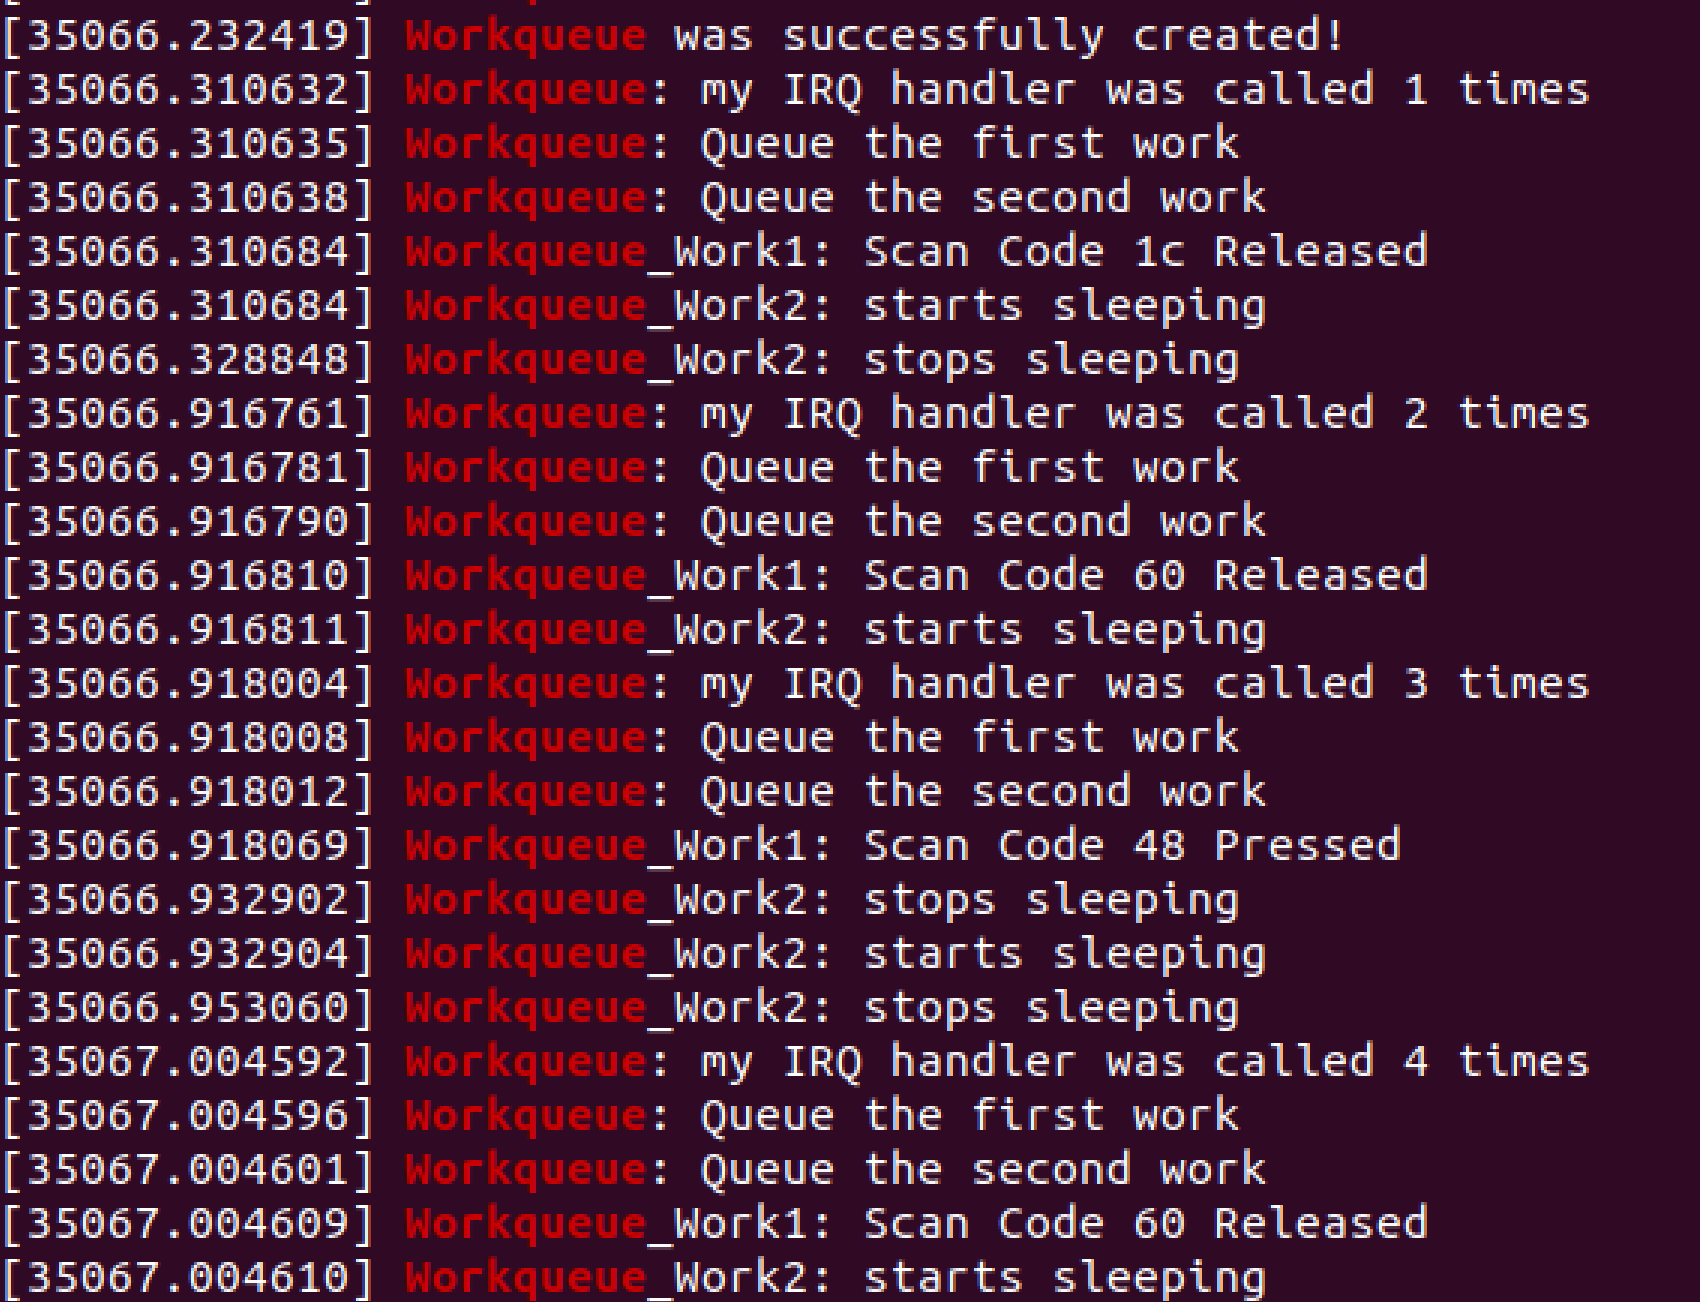
\includegraphics[scale=0.5]{pics/Res.png}
		
			Рис 1:  Результат работы программы 
\end{center}


\end{document}